\documentclass[10pt]{article}
\usepackage{fontspec}
\usepackage{polyglossia}
\setdefaultlanguage{french}
\usepackage[a4paper,margin=2cm]{geometry}
\usepackage{url,hyperref}
\usepackage{siunitx}
\usepackage{schemabloc}
\usepackage{listings}
\usepackage{auto-pst-pdf}
\usepackage{pst-circ}
\usepackage{soul}
\usepackage{verbatim}
\usepackage{lmodern}
\usepackage{tikz}
\usepackage[european,cuteinductors,siunitx]{circuitikz}
\usepackage{xunicode,xltxtra}
\usepackage{graphicx}
\usepackage{amsmath}
\usepackage{minted}
\usepackage{multicol}
\usepackage{float}
\floatplacement{figure}{H}

\lstset {
    language=Matlab,
    basicstyle=\footnotesize,
    numbers=left,
    numberstyle=\footnotesize,
    stepnumber=1,
    numbersep=5pt,
    backgroundcolor=\color{white},
    showspaces=false,
    showstringspaces=true,
    showtabs=true,
    frame=single,
    tabsize=4,
    captionpos=b,
    breaklines=true,
    breakatwhitespace=true,
    title=\lstname,
}

\renewcommand{\thesubsection}{\thesection .\alph{subsection}}

\title{
\includegraphics{../../../images/inp-enseeiht} \\ ~ \\ ~ \\ ~ \\ ~ \\ BE Fonction Hyperfréquences}
\author{Mathieu Couffinhal, Guilhem Saurel}
\date{}

\begin{document}
\begin{titlepage}
    \maketitle
    \tableofcontents
\end{titlepage}

\section{Étude de deux briques de base : tronçon de ligne et admittance parallèle.}
\subsection{}
\begin{itemize}
    \item[•] \textit{Identifier la matrice \textbf{ABCD} du quadripôle, puis déduire la matrice \textbf{abcd} en prenant comme impédance de référence des accès \textbf{$Z_c$}. Programmer sous MATLAB cette dernière en fonction de \textbf{$Z_c$}, \textbf{$v_p$}, \textbf{d}, et de la fréquence de travail \textbf{$f_0$} ; (\ul{valeurs initiales} : \textbf{$Z_c$} = $50\Omega$ ; \textbf{$v_p$} = $2E8m/s$ ; \textbf{d} = $2m$ ; \textbf{$f_0$} = $13.56MHz$).}
        \begin{center}
            \begin{pspicture}(7,3)
                \pnode(1,2.5){A}
                \pnode(1,0.5){B}
                \pnode(5,2.5){C}
                \pnode(5,0.5){D}
                \pnode(0,2.5){a}
                \pnode(0,0.5){b}
                \pnode(6,2.5){c}
                \pnode(6,0.5){d}
                \quadripole(A)(B)(C)(D){ABCD}
                \tension(B)(A){$V_1$}
                \tension[labeloffset=-0.5](D)(C){$V_2$}
                \wire[intensitylabel=$I_1$](a)(A)
                \wire(b)(B)
                \wire[intensitylabel=$I_2$,intensitylabeloffset=-0.5](c)(C)
                \wire(d)(D)
            \end{pspicture}
        \end{center}

        On sait que :

        \[
            \begin{pmatrix}
                V_1 \\
                I_1
            \end{pmatrix}
            =
            \begin{pmatrix}
                A & B \\
                C & D
            \end{pmatrix}
            \begin{pmatrix}
                V_2 \\
                -I_2
            \end{pmatrix}
        \]

        D'où

        \begin{eqnarray}
            V_1 &=& A V_2 - B I_2 \\
            I_1 &=& C V_2 - D I_2
        \end{eqnarray}

        Or, dans une ligne de transmissions, 

        \begin{eqnarray}
            V(z) &=& V^+ e^{+\gamma z} +V^- e^{-\gamma z} \\
            I(z) &=& \cfrac{V^+ e^{+\gamma z} -V^- e^{-\gamma z}}{Z_c}
        \end{eqnarray}

        Donc, dans notre cas, par application directe, et en prenant classiquement l'origine à l'utilisation :

        \begin{eqnarray}
            V_2 &=& V^+ + V^- \\
            V_1 &=& V^+ e^{+\gamma d} +V^- e^{-\gamma d} \\
            I_2 &=& \cfrac{V^+ -V^- }{Z_c}\\
            I_1 &=& \cfrac{V^+ e^{+\gamma d} -V^- e^{-\gamma d}}{Z_c}
        \end{eqnarray}

        On en déduit

        \begin{eqnarray}
            (1.5) \& (1.7) \Rightarrow V^- &=& \cfrac{Z_c I_2 + V_2}{2}
        \end{eqnarray}

        Donc, en injectant (1.9) dans (1.6),

        \begin{eqnarray}
            V_1 &=& (V_2 - V^-) e^{+\gamma d} + V^- e^{-\gamma d} \nonumber \\
            &=& (V_2 - \cfrac{Z_c I_2 + V_2}{2}) e^{+\gamma d} + \cfrac{Z_c I_2 + V_2}{2} e^{-\gamma d} \nonumber \\
            &=& V_2 \left(\cfrac{e^{\gamma d} + e^{-\gamma d}}{2}\right) - I_2 Z_c \left(\cfrac{e^{\gamma d} - e^{-\gamma d}}{2}\right) \nonumber \\
            &=& V_2 \cosh(\gamma d) - I_2 Z_c \sinh(\gamma d)
        \end{eqnarray}

        D'où, par identification entre (1.10) et (1.1),

        \begin{eqnarray}
            A &=& \cosh(\gamma d) \\
            B &=& Z_c \sinh(\gamma d)
        \end{eqnarray}

        Et, de la même manière,

        \begin{eqnarray}
            C &=& Y_c \sinh(\gamma d) \\
            D &=& \cosh(\gamma d)
        \end{eqnarray}

        On en déduit la matrice \textbf{abcd} :

        \begin{eqnarray}
            a &=& A \\
            b &=& \cfrac{B}{Z_c} \\
            c &=& \cfrac{B}{Y_c} \\
            d &=& D
        \end{eqnarray}

        Ce qui donne, sous MATLAB :
        %\lstinputlisting[language=Matlab,lastline=20]{sources/1a.m}
        \inputminted[linenos]{matlab}{src/1a.m}

    \item[•] \textit{Déduire de la matrice \textbf{abcd} la matrice impédance réduite et la matrice S ; programmer ces relations de passage sous forme de fichier \textbf{*.m} ; vérifier la nature réciproque et sans perte de ce quadripôle.}

        On sait que
        \[
            \begin{pmatrix}
                v_1 \\
                v_1
            \end{pmatrix}
            =
            \begin{pmatrix}
                z_{11} & z_{12} \\
                z_{21} & z_{22}
            \end{pmatrix}
            \begin{pmatrix}
                i_1 \\
                i_2
            \end{pmatrix}
        \]

        D'où

        \begin{eqnarray}
            v_1 &=& z_{11} i_1 + z_{12} i_2 \\
            v_2 &=& z_{21} i_1 + z_{22} i_2
        \end{eqnarray}

        Or, on rappelle (1.1) et (1.2) pour une impédance réduite :

        \begin{eqnarray}
            v_1 &=& a v_2 - b i_2 \\
            i_1 &=& c v_2 - d i_2
        \end{eqnarray}

        Donc

        \begin{eqnarray}
            (1.21) \Rightarrow c v_2 &=& i_1 + d i_2 \nonumber \\
            \Rightarrow v_2 &=& \cfrac{1}{c} i_1 + \cfrac{d}{c} i_2
        \end{eqnarray}

        D'où, par identification, entre (1.20) et (1.23), 

        \begin{eqnarray}
            z_{21} &=& \cfrac{1}{c} \\
            z_{22} &=& \cfrac{d}{c}
        \end{eqnarray}

        On remplace alors (1.23) dans (1.21) :

        \begin{eqnarray}
            v_1 &=& a \left( \cfrac{1}{c} i_1 + \cfrac{d}{c} i_2 \right) - b i_2 \nonumber \\
            &=& \cfrac{a}{c} i_1 + \cfrac{a d - b c}{c} i_2
        \end{eqnarray}

        Puis en identifiant (1.19) et (1.26) :

        \begin{eqnarray}
            z_{11} &=& \cfrac{a}{c} \\
            z_{12} &=& \cfrac{a d - b c}{c}
        \end{eqnarray}

        On en déduit les paramètres S :

        \begin{eqnarray}
            S_{11} &=& \cfrac{A + \cfrac{B}{Z_c} - C Z_c - D}{A+\cfrac{B}{Z_c} +C Z_c +D} \\
            S_{12} &=& 2 \cfrac{A D - B C}{A+\cfrac{B}{Z_c} +C Z_c +D} \\
            S_{21} &=& \cfrac{2}{A+\cfrac{B}{Z_c} +C Z_c +D} \\
            S_{22} &=& \cfrac{-A +\cfrac{B}{Z_c} + C Z_c +D}{A+\cfrac{B}{Z_c} +C Z_c +D}
        \end{eqnarray}

        On vérifie la nature réciproque de ce quadripole car le déterminant de la matrice S est égal à 1.

        De plus, cette matrice ne peut etre que sans pertes : en effet, jusqu'ici, tous les calculs ont été faits avec un certain $\gamma$, mais les données du problème ne nous permettent de déduire que $\gamma = j \beta = \cfrac{j \omega}{v_\varphi}$, comme est codée la variable "g" dans le fichier .m depuis le début.

        On programme ces relations de passage sous forme de fichier \textbf{*.m} :
        %\lstinputlisting[language=Matlab,firstline=21,lastline=43,firstnumber=21]{sources/1a.m}
        \inputminted[linenos]{matlab}{src/1a.m}


    \item[•] \textit{Montrer que les éléments de cette matrice dépendent de la fréquence en traçant la partie léelle de \textbf{a} et la partie imaginaire de \textbf{b} avec \textbf{$f_0$} variant de 100MHz à 500MHz.}
    %\lstinputlisting[language=Matlab,firstline=44,firstnumber=44]{sources/1a.m}
    \inputminted[linenos]{matlab}{src/1a.m}

    %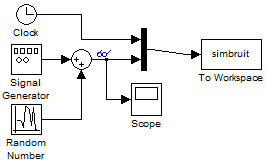
\includegraphics[width=\linewidth,height=6cm]{images/1a}

\end{itemize}

\subsection{}
\begin{itemize}
    \item[•] \textit{À l'aide de la matrice impédance, déterminer l'impédance vue par le générateur : $Z_E$}.

        \begin{center}
            \begin{pspicture}(7,3)
                \pnode(1,2.5){A}
                \pnode(1,0.5){B}
                \pnode(5,2.5){C}
                \pnode(5,0.5){D}
                \pnode(0,2.5){a}
                \pnode(0,0.5){b}
                \pnode(6,2.5){c}
                \pnode(6,0.5){d}
                \quadripole(A)(B)(C)(D){Z}
                \tension(B)(A){$V_1$}
                \tension[labeloffset=-0.5](D)(C){$V_2$}
                \wire[intensitylabel=$I_1$](a)(A)
                \wire(b)(B)
                \wire[intensitylabel=$I_2$,intensitylabeloffset=-0.5](c)(C)
                \wire(d)(D)
                \resistor[labeloffset=-1](d)(c){$Z_{ant}$}
            \end{pspicture}
        \end{center}

        Donc on a

        \begin{eqnarray}
            V_1 &=& Z_{11} I_1 + Z_{12} I_2 \\
            V_2 &=& Z_{21} I_1 + Z_{22} I_2 \\
            V_2 &=& - Z_{ant} I_2 \\
            Z_E &=& \cfrac{V_1}{I_1}
        \end{eqnarray}

        Donc en égalisant (1.34) et (1.35),

        \begin{eqnarray}
            -Z_{ant} I_2 &=& Z_{21} I_1 + Z_{22} I_2 \nonumber \\
            \Leftrightarrow -Z_{21} I_1 &=& \left(Z_{22} + Z_{ant}\right) I_2 \nonumber \\
            \Leftrightarrow I_2 &=& \cfrac{-Z_{21}}{Z_{22} + Z_{ant}} I_1
        \end{eqnarray}

        Donc en injectant (1.37) dans (1.33) de manière à identifier avec (1.36),

        \begin{eqnarray}
            V_1 &=& Z_{11} I_1 + Z_{12} \cfrac{-Z_{21}}{Z_{22} + Z_{ant}} I_1 \nonumber \\
            \Leftrightarrow Z_E &=& Z_{11} - \cfrac{Z_{12} Z_{21}}{Z_{22} + Z_{ant}}
        \end{eqnarray}

    \item[•] \textit{Déterminer la tension et le courant à l'entrée de la ligne : $V_1$, $I_1$ ; puis déduire la tension et le courant à la sortie de la ligne ($V_2$, $I_2$) à l'aide de la matrice \textbf{ABCD}.}

        Si la puissance disponible est de $P_d = 33 dBm$, la puissance disponible en Watts vaut $P_d = 10^{6.3}W$.

        Si le générateur était chargé par $50 \Omega$, on aurait un pont diviseur par 2: $P_d = \cfrac{1}{2} \cfrac{|E_g|^2}{4R_c} \Rightarrow E_g = \sqrt{8 R_c Pd}$, ce qui est la puissance maximale.

        De plus

        \begin{eqnarray}
            V_1 &=& \cfrac{E_g Z_E}{Z_E+R_c}
        \end{eqnarray}

        Donc

        \begin{eqnarray}
            I_1 &=& \cfrac{V_1}{Z_E} = \cfrac{E_g}{Z_E+R_c}
        \end{eqnarray}

        Et, à l'aide de la matrice ABCD, on en déduit : 
        \[
            \begin{pmatrix}
                V_2 \\
                -I_2
            \end{pmatrix}
            =
            \begin{pmatrix}
                A & B \\
                C & D
            \end{pmatrix}
            \begin{pmatrix}
                V_1 \\
                I_1
            \end{pmatrix}
        \]

        D'où

        \begin{eqnarray}
            V_2 &=& A V_1 + B I_1 \nonumber \\
            &=& \cfrac{E_g Z_E}{Z_E+R_c} \cosh(\gamma d) + \cfrac{E_g}{Z_E+R_c} Z_c \sinh(\gamma d)\\
            I_2 &=& -C V_1 - D I_1 \nonumber \\
            &=& - Y_c \cfrac{E_g Z_E}{Z_E+R_c} \sinh(\gamma d) - \cfrac{E_g}{Z_E+R_c} \cosh(\gamma d)
        \end{eqnarray}

    \item[•] \textit{Déduire $a_1$, $b_1$, $a_2$ et $b_2$ à partir de la connaissance de $V_1$, $I_1$, $V_2$, $I_2$.}

        On a alors :

        \begin{eqnarray}
            a_1 = \cfrac{ V_1 + Z_c I_1}{2} \\
            b_1 = \cfrac{ V_1 - Z_c I_1}{2} \\
            a_2 = \cfrac{ V_2 + Z_c I_2}{2} \\
            b_2 = \cfrac{ V_2 - Z_c I_2}{2}
        \end{eqnarray}

    \item[•] \textit{Calculer les coefficients de réflexion à l'entrée et à la sortie de l'interconnexion, la puissance dissipée dans l'antenne ( correspondant à la puissance rayonnée), la puissance réfléchie vers le générateur, ainsi que la puissance développée par le générateur. Calculer les pertes d'insertion \textbf{IL} (\emph{Insertion Loss}) et les pertes en réflexions \textbf{RL} (\emph{Return Loss}) ; conclure.}

        Par définition, on a les coefficients de réflexion suivants :

        \begin{eqnarray}
            \Gamma_e &=& \cfrac{b_1}{a_1} \\
            \Gamma_s &=& \cfrac{b_2}{a_2}
        \end{eqnarray}

        Toujours par définition, la puissance dissipée dans l'antenne vaut :

        \begin{eqnarray}
            P_{ray} &=& \cfrac{V_2 I_2^\ast}{2}
        \end{eqnarray}

        La puissance réfléchie vers le générateur correspond à la puissance de l'onde $b_1$, qui est celle réfléchie vers le générateur :

        \begin{eqnarray}
            P_{ref} &=& \cfrac{|b_1|^2}{2}
        \end{eqnarray}

        La puissance développée par le générateur est donc logiquement la somme de la puissance rayonnée et de celle réfléchie vers le générateur, vu que la ligne de transmission est sans pertes :

        \begin{eqnarray}
            P_f &=&  \cfrac{V_2 I_2^\ast + |b_1|^2}{2}
        \end{eqnarray}

        Il ne reste plus qu'à calculer les pertes d'insertion et en réflexion :

        \begin{eqnarray}
            IL &=& 10 \log \cfrac{P_d}{P_f} \\
            RL &=& 10 \log \cfrac{P_d}{P_{ref}}
        \end{eqnarray}

\end{itemize}

Remarque : Dans cette partie, il n'y avait rien à faire en MATLAB, mais nous nous en sommes rendu compte qu'après l'avoir tout de même fait, donc voici le fichier, en bonus :
%\lstinputlisting[language=Matlab]{sources/1b.m}
\inputminted[linenos]{matlab}{src/1b.m}

\subsection{}
\begin{itemize}
    \item[•] \textit{Programmer sa matrice \textbf{abcd} ; (\ul{valeurs initiales} : une capacitance de $10pF$ en parallèle avec une self de $3.36nH$ et une résistance de $4k\Omega$ ; \textbf{$Z_c$} = $50\Omega$ ; \textbf{$f_0$} = $500MHz$)}
        \begin{eqnarray*}
            Y_p &=& j 3.36 \times 10^{-9} \omega + \cfrac{1}{j 10 \times 10^{-12} \omega} + \cfrac{1}{4\times 10^3}
        \end{eqnarray*}

        Or la matrice d'un dipole $Y_p$ en parallèle est assez simple :

        \begin{center}
            \begin{pspicture}(3,3)
                \pnode(0,0.5){a}
                \pnode(0,2.5){b}
                \pnode(1,0.5){c}
                \pnode(1,2.5){d}
                \pnode(2,0.5){e}
                \pnode(2,2.5){f}
                \wire[intensitylabel=$I_1$](b)(d)
                \wire[intensitylabel=$I_2$,intensitylabeloffset=-0.5](f)(d)
                \wire(a)(e)
                \resistor[labeloffset=0](d)(c){$Y_p$}
                \tension[labeloffset=0.5](a)(b){$V_1$}
                \tension[labeloffset=-0.5](e)(f){$V_2$}
            \end{pspicture}
        \end{center}

        On a directement

        \begin{eqnarray}
            V_1 &=& V_2 = \cfrac{I_1 + I_2}{Y_p}
        \end{eqnarray}

        D'où la représentation sous MATLAB suivante :

        %\lstinputlisting[language=Matlab,lastline=8]{sources/1c.m}
        \inputminted[linenos]{matlab}{src/1c.m}

    \item[•] \textit{En faisant varier la fréquence entre $500MHz$ et $1GHz$, calculer à l'aide du programme de passage développé en \emph{1.a} la variation du coefficient de réflexion et du coefficient de transmission en fonction de la fréquence ; trancer sous MATLAB la variation de $S_{11}$ à l'aide des commandes \textbf{plot} et \textbf{smith} ; tracer également la variation de $S_{21}$ à l'aide de \textbf{plot}.}

        Il nous faut la relation de mise en chaine de deux matrices \textbf{ABCD} : 

        \begin{center}
            \begin{pspicture}(13,3)
                \pnode(0,2.5){a}
                \pnode(0,0.5){b}
                \pnode(1,2.5){A}
                \pnode(1,0.5){B}
                \pnode(5,2.5){C}
                \pnode(5,0.5){D}
                \pnode(6,2.5){c}
                \pnode(6,0.5){d}
                \pnode(7,2.5){E}
                \pnode(7,0.5){F}
                \pnode(11,2.5){G}
                \pnode(11,0.5){H}
                \pnode(12,2.5){g}
                \pnode(12,0.5){h}
                \quadripole(A)(B)(C)(D){$A_1 B_1 C_1 D_1$}
                \quadripole(E)(F)(G)(h){$A_2 B_2 C_2 D_2$}
                \tension(B)(A){$V_1$}
                \tension[labeloffset=-0.5](d)(c){$V'$}
                \tension[labeloffset=-0.5](H)(G){$V_2$}
                \wire[intensitylabel=$I_1$](a)(A)
                \wire(b)(B)
                \wire[intensitylabel=$I'$,intensitylabeloffset=-0.5](c)(C)
                \wire(D)(F)
                \wire[intensitylabel=$-I'$](c)(E)
                \wire[intensitylabel=$I_2$,intensitylabeloffset=-0.5](g)(G)
                \wire(h)(H)
            \end{pspicture}
        \end{center}

        D'où

        \begin{eqnarray}
            V_1 &=& A_1 V' - B_1 I' \\
            I_1 &=& C_1 V' - D_1 I' \\
            V' &=& A_2 V_2 - B_2 I_2 \\
            -I' &=& C_2 V_2 - D_2 I_2
        \end{eqnarray}

        Donc, en substituant (1.56) et (1.57) dans (1.54) et (1.55),

        \begin{eqnarray}
            V_1 &=& A_1 A_2 V_2 - A_1 B_2 I_2 + B_1 C_2 V_2 - B_1 D_2 I_2 \nonumber \\
            &=& (A_1 A_2 + B_1 C_2) V_2 - (A_1 B_2 + B_1 D_2) I_2 \\
            I_1 &=& C_1 A_2 V_2 - C_1 B_2 I_2 + D_1 C_2 V_2 - D_1 D_2 I_2 \nonumber \\
            &=& (C_1 A_2 +D_1 C_2) V_2 - (C_1 B_2 + D_1 D_2) I_2
        \end{eqnarray}

        Pour avoir la matrice de chaîne équivalente à la chaîne de deux matrices de chaîne, il suffit donc de multiplier ces matrices.

        On programme donc la matrice \textbf{abcd} correspondant à la chaine des matrices du circuit d'adaptation et de la ligne de transmission, puis on traduit le tout en une matrice S qui dépend de la fréquence : 

        \newpage
        %\lstinputlisting[language=Matlab,firstline=10,firstnumber=10]{sources/1c.m}
        \inputminted[linenos]{matlab}{src/1c.m}

        %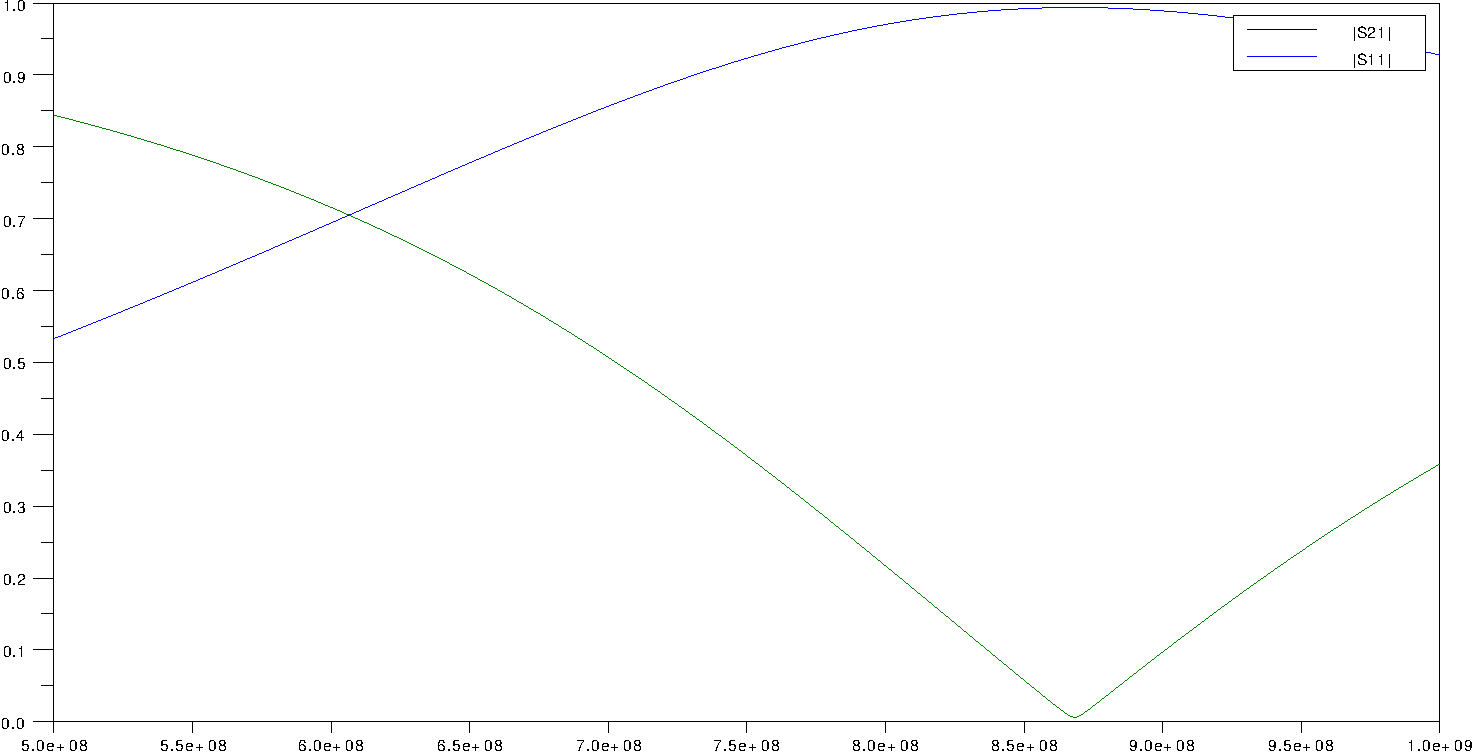
\includegraphics[width=\linewidth,height=8cm]{images/1c}

\end{itemize}

\subsection{Modèle d'un stub court-circuité en parallèle.}
De la même manière, en remplaçant simplement $Y_p$ par $Z_c j \tan(\beta l)$

%\lstinputlisting[language=Matlab]{sources/1d.m}
\inputminted[linenos]{matlab}{src/1d.m}

%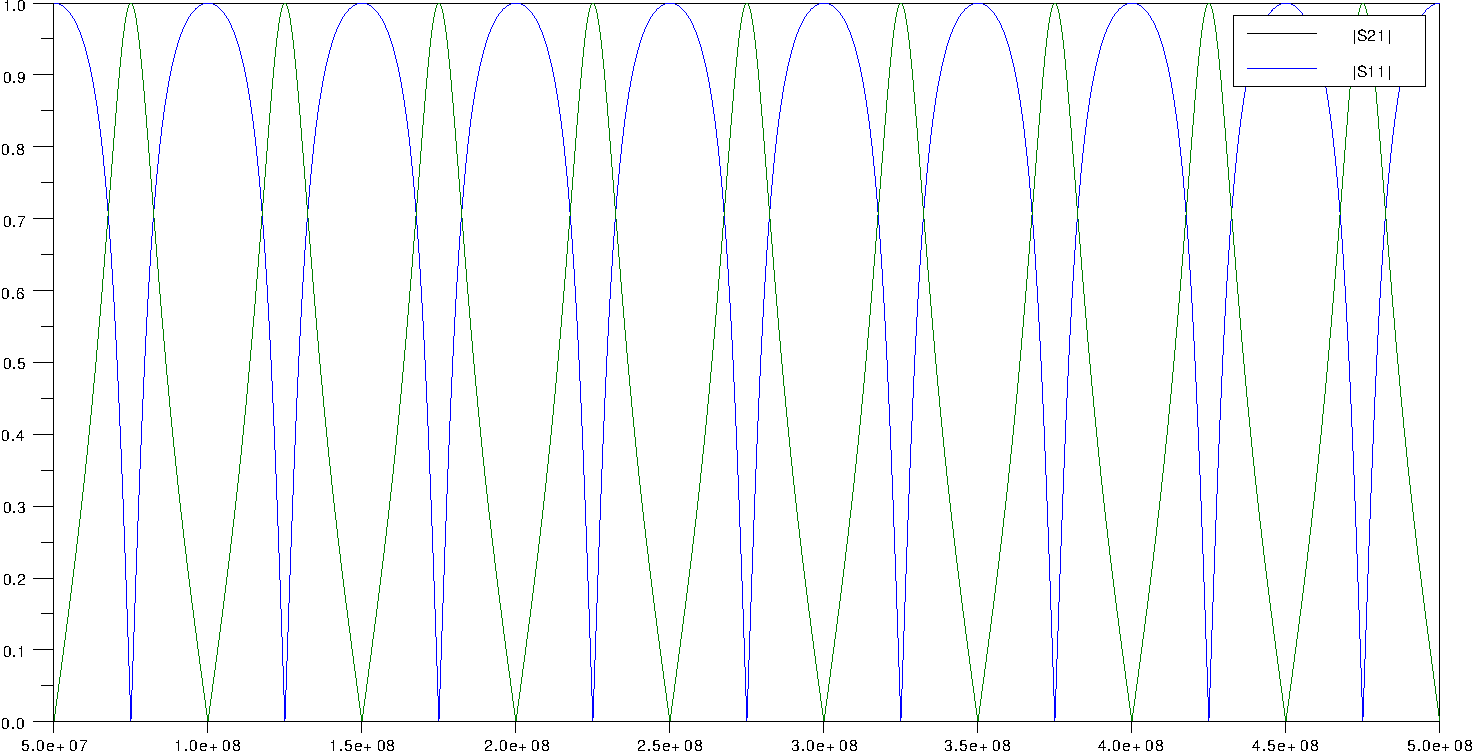
\includegraphics[width=\linewidth,height=8cm]{images/1d}

\section{Amélioration du système d'antenne. Adaptation d'antenne.}
\subsection{Étude du circuit d'adaptation.}
Les deux solutions sont directement données par les applets java du site \verb|http://amanogawa.com| :

\begin{center}
    %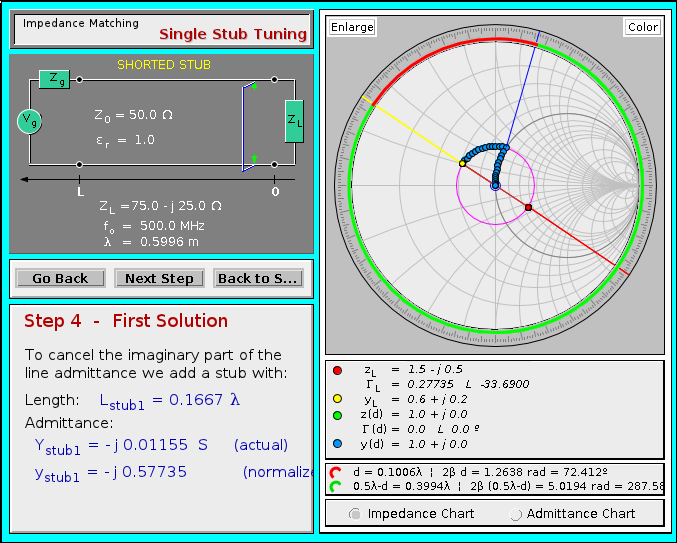
\includegraphics[height=7cm]{images/s1}

    %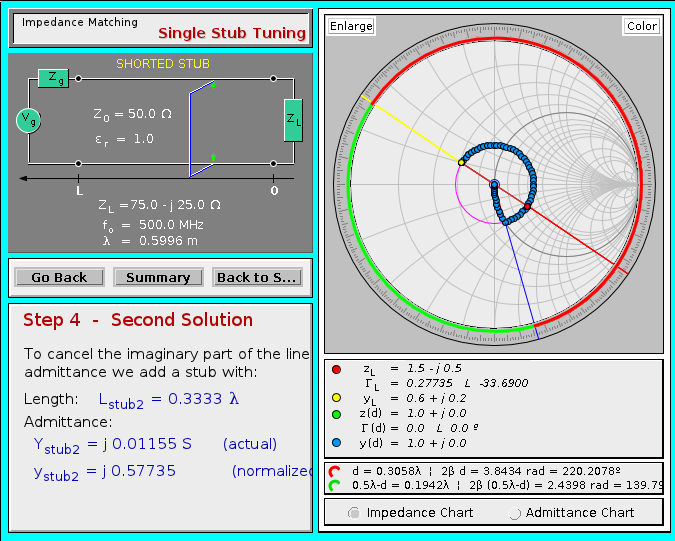
\includegraphics[height=7cm]{images/s2}
\end{center}
\subsection{}

D'après Amanogawa, il faut mettre une ligne de transmission de longueur $d=0.1006 \lambda = 60.3mm$ après la charge, puis un simple stub de longueur $L=0.1667\times 0.5996=99.9mm$, et on rajoutera notre ligne de 2m.

On a donc directement le code MATLAB suivant :

%\lstinputlisting[language=Matlab]{sources/2b.m}
\inputminted[linenos]{matlab}{src/2b.m}

\subsection{}
Comme précédement, on peut étudier les pertes en réflexion en traçant $S_{11}$ en fonction de la fréquence. On peut également tracer la puissance réfléchie ($\cfrac{|b_1|^2}{2}$) et la puissance rayonnée ($P_{ray} = \cfrac{V_2I_2^\ast}{2}$) en fonctiond de cette fréquence.

%\lstinputlisting[language=Matlab]{sources/2c.m}
\inputminted[linenos]{matlab}{src/2c.m}
\end{document}
